\chapter{Data Generation}
\label{data-generation}

The obtained data solely included information about meal orders, without any additional details about the distribution centers' locations or the ingredients incorporated in each meal. To effectively model the VRPC step, additional data was required. To address this data gap, both machine learning and statistical methodologies were utilized to generate a suitable dataset. The generation process utilized the hints provided in the original dataset to create data that was as plausible as possible.

Section~\ref{datagen-ingredient-composition} outlines the methodology utilized to generate a realistic ingredient list for each meal,
Section~\ref{datagen-distribution-center-locations} details the approach employed to randomly generate distribution center locations.

\section{Ingredient composition}
\label{datagen-ingredient-composition}
In order to generate the ingredient composition for each meal, we employed the use of ChatGPT, a sophisticated language model that is capable of generating text based on a given prompt. We sent the name for each meal and we asked how many grams of each ingredients are required, in order to ensure the accuracy and plausibility of the generated data, we implemented a human supervision step.

While the generated data did contain some errors, expecially in the weight of the ingredients, the supervisor could easily find and correct these, producing an high quality, mostly plausible ingredient list directly in CSV format. The following paste will contain an example of the generated data:


\begin{verbatim}
    meal_id,ingredient,weight_grams
    Pasta al Pesto,Pasta,100
    Pasta al Pesto,Basil Pesto,50
    Pasta al Pesto,Parmesan Cheese,20
    Pasta al Pesto,Pine Nuts,20
    Pasta al Pesto,Garlic,10
    Chicken Rice Bowl,Chicken,200
    Chicken Rice Bowl,White Rice,150
    Chicken Rice Bowl,Red Bell Pepper,50
    Chicken Rice Bowl,Cucumber,50
    Chicken Rice Bowl,Carrot,50
    Chicken Rice Bowl,Onion,20
    Chicken Rice Bowl,Soy Sauce,15
    Chicken Rice Bowl,Honey,10
\end{verbatim}

\section{Distribution center locations}
\label{datagen-distribution-center-locations}
The original data provides only partial information about the location of each facility, specifying only the city and region through anonymized IDs. Despite this limitation, we use the available data to generate plausible location positions for the centers. Instead of generating random positions for the centers directly, we first generate regions, then cities, and finally centers. This hierarchical approach enables us to use the known city and region information to inform the positions of the centers by relative positioning.

To ensure that the generated locations are feasible, we have implemented two additional constraints. Firstly, we ensure that the regions, cities, and centers are a minimum distance apart. If this criterion is not met, the positions are regenerated until the minimum distance is achieved. Secondly, we sample the distribution of centers from a normal distribution, with the variance varying based on the size of the city they are located in. This means that larger cities have more sparse facilities, while smaller cities have facilities located closer to their center.

The central depot is located using a similar method to that used for the centers. However, instead of choosing a specific city for the depot, we randomly select a city from among the available options, with a bias towards larger cities. This ensures that the central depot is strategically placed to enable efficient distribution to the centers located throughout the region.

The resulting distribution can be visualized in Figure~\ref{fig:center_locations}, depicting both regions, cities, centers and the central Depot.


\begin{figure}[tb]
    \centering
    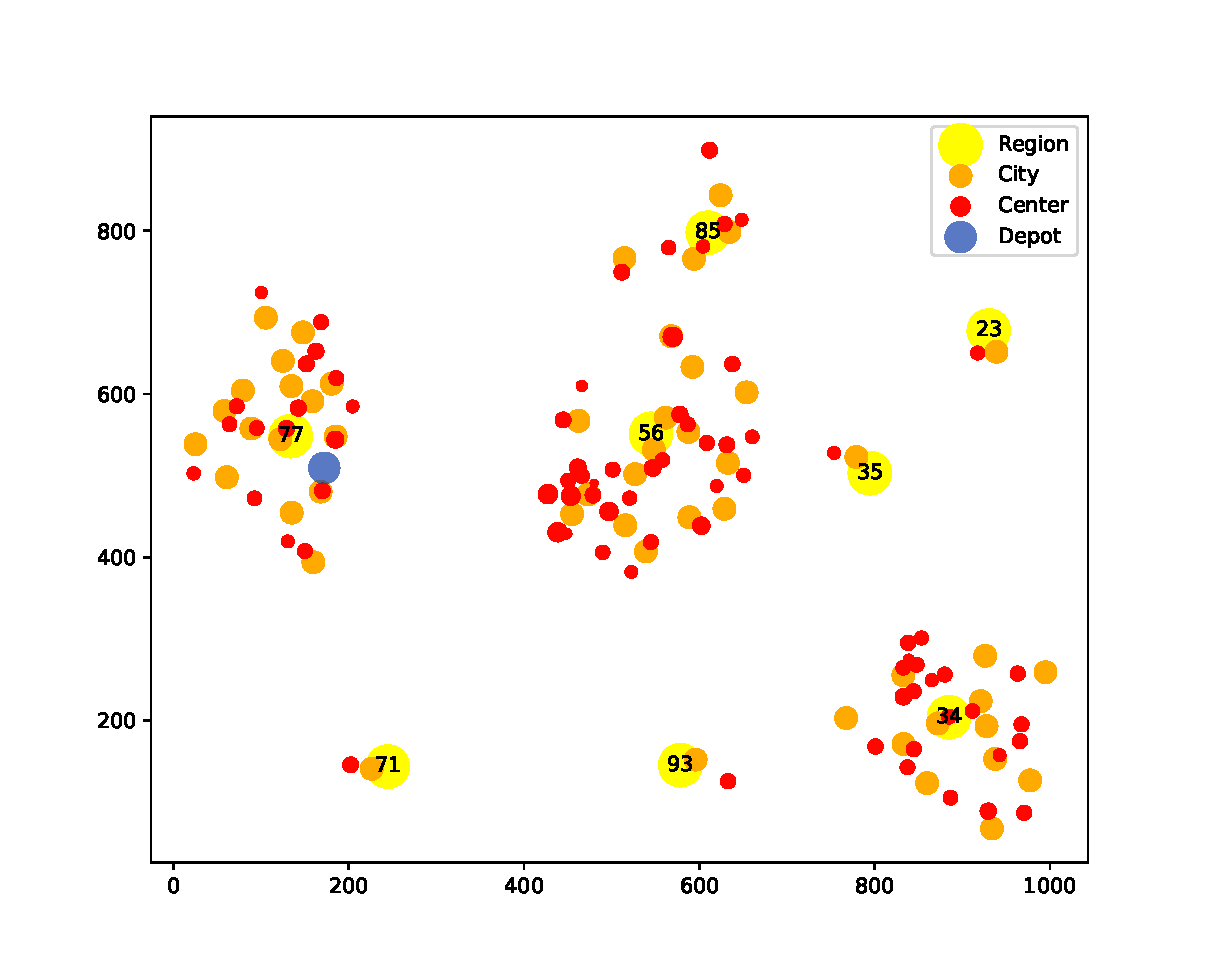
\includegraphics[width=1\columnwidth]{figures/center_locations.pdf}
    \caption{Locations of the centers in a square 2D grid}
  \label{fig:center_locations}
\end{figure}
